\documentclass[12pt]{article}
\setlength{\oddsidemargin}{0in}
\setlength{\evensidemargin}{0in}
\setlength{\textwidth}{6.5in}
\setlength{\parindent}{0in}
\setlength{\parskip}{\baselineskip}
\usepackage{amsmath,amsfonts,amssymb}
\usepackage{graphicx}
\usepackage{enumitem}
\usepackage[]{algorithmicx}
\usepackage{amsthm}
\usepackage{fancyhdr}
\pagestyle{fancy}
\setlength{\headsep}{36pt}
\usepackage{tkz-berge}
\usetikzlibrary{positioning, automata}

\usepackage{hyperref}

\theoremstyle{remark}
\newtheorem*{solution}{Solution}

\newcommand{\makenonemptybox}[2]{%
%\par\nobreak\vspace{\ht\strutbox}\noindent
\item[]
\fbox{% added -2\fboxrule to specified width to avoid overfull hboxes
% and removed the -2\fboxsep from height specification (image not updated)
% because in MWE 2cm is should be height of contents excluding sep and frame
\parbox[c][#1][t]{\dimexpr\linewidth-2\fboxsep-2\fboxrule}{
  \hrule width \hsize height 0pt
  #2
 }%
}%
\par\vspace{\ht\strutbox}
}
\makeatother

\begin{document}

\lhead{{\bf CSCI 3104, Algorithms \\ Problem Set 10a (25 points)} }
\rhead{Name: \fbox{Michael Rogers} \\ ID: \fbox{105667404} \\ {\bf Profs.\ Hoenigman \& Agrawal\\ Fall 2019, CU-Boulder}}
\renewcommand{\headrulewidth}{0.5pt}

\phantom{Test}

\begin{small}
\textit{Advice 1}:\ For every problem in this class, you must justify your answer:\ show how you arrived at it and why it is correct. If there are assumptions you need to make along the way, state those clearly.
\vspace{-3mm} 

\textit{Advice 2}:\ Verbal reasoning is typically insufficient for full credit. Instead, write a logical argument, in the style of a mathematical proof.\\
\vspace{-3mm} 

\textbf{Instructions for submitting your solution}:
\vspace{-5mm} 

\begin{itemize}
	\item The solutions \textbf{should be typed} and we cannot accept hand-written solutions. \href{http://ece.uprm.edu/~caceros/latex/introduction.pdf}{Here's a short intro to Latex.}
	\item You should submit your work through \href{https://www.gradescope.com/courses/59294}{\textbf{Gradescope}} only.
	\item If you don't have an account on it, sign up for one using your CU email. You should have gotten an email to sign up. If your name based CU email doesn't work, try the identikey@colorado.edu version. 
	\item Gradescope will only accept \textbf{.pdf} files (except for code files that should be submitted separately on Gradescope if a problem set has them) and \textbf{try to fit your work in the box provided}. 
	\item You cannot submit a pdf which has less pages than what we provided you as Gradescope won't allow it. 
\end{itemize}
\vspace{-4mm} 
\end{small}

\hrulefill
\pagebreak


\begin{enumerate}

\item (11 pts) Solve the following based on the given intervals.
\begin{center}
\begin{tabular}{c|c|c}
Event Index & Interval & Value\\ \hline
1 & $[1, 10]$ & 10\\ 
2 & $[11, 20]$  & 5\\
3 & $[21, 30]$  & 15\\
4 & $[9, 12]$ & 7\\
5 & $[19, 22]$ & 8
\end{tabular}
\end{center}

\begin{enumerate}

\item (2.5 pts) For the given set of requests with a start and finish time and a value, what is $p(j)$ for each request $j$?

\begin{solution}Function defining $p(j)$: \\
First we must sort the events by finish time, then: \\
$p(j) =$ number of requests i not overlapping with request $j$, where $i < j$
\end{solution}

\item (1.5 pts) Assume you are given a greedy algorithm for the weighted interval scheduling problem that selects the requests in descending order of their value, i.e. highest valued requests are selected first. Provide an example set of intervals where this approach won't produce the optimal solution.
\begin{solution}
\begin{center}
\begin{tabular}{c|c|c}
Event Index & Interval & Value\\ \hline
1 & $[1, 10]$ & 11\\ 
2 & $[2, 5]$  & 7\\
3 & $[6, 7]$  & 8\\
4 & $[7, 9]$ & 5
\end{tabular}
\end{center}
This greedy algorithm would select event 1 which has the highest value, but it can no longer select any other events because they all take place within 1. The optimal would have been \{2, 3, 4\} which total 20 in value.
\end{solution}

\pagebreak
\item (2 pts) In the following recursive formula for the weighted interval scheduling problem in Question 1, how many recursive calls are there to \textit{WISNoMem}? Show the recursion tree to support your answer.
\begin{verbatim}
WISNoMem(j) {
    if (j == 0) 
        return 0
    else 
        return max(WISNoMem(j-1), v[j] + WISNoMem(p[j]))
}
\end{verbatim}

\begin{solution}
First, the events in the table must be sorted by finish time\\
The WISNoMem function will run 30 times. If we used a DP memoization approach the function would only run 5 times as it would store the values of WNM(3), WNM(2), WNM(1), and WNM(0). \\
\begin{center}
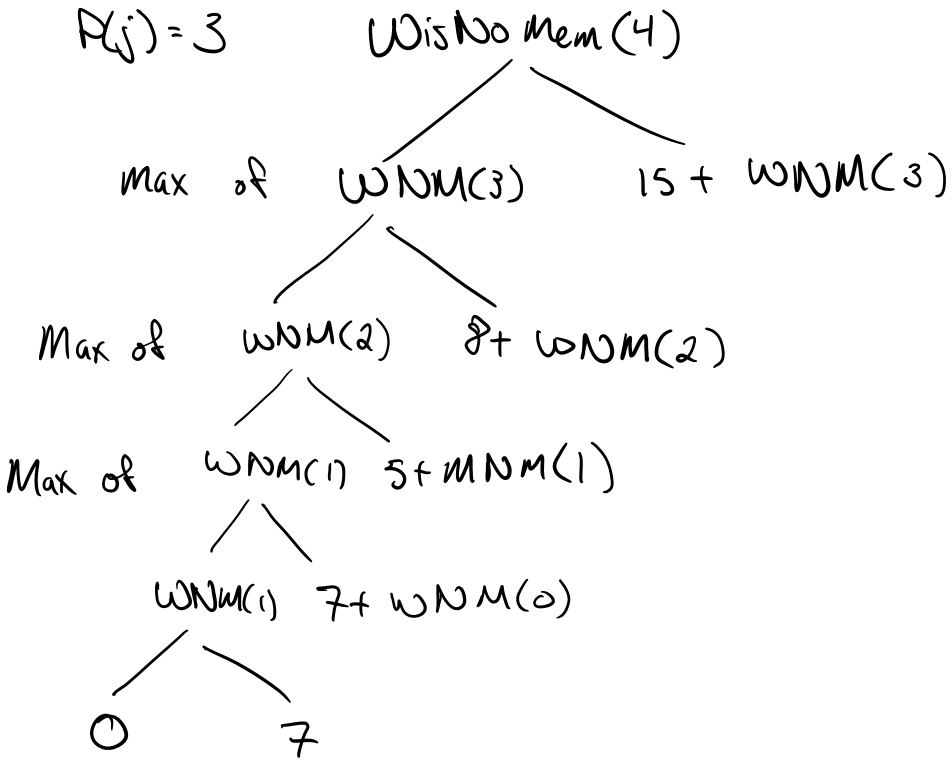
\includegraphics[scale = 0.6]{PS10a_Q1c.png}
\end{center}
\end{solution}

\pagebreak
\item (3 pts) Using the bottom-up iterative algorithm presented in lecture, show the $OPT(j)$ values for all requests. Also draw the arrows to show the previous sub-problem you used to fill an entry. 
\begin{solution}
1: Event 1 \\
2: Event 1 \\
3: Event 1 \\
4: Event 1 \\
5: Event 5
\end{solution}
\item (2 pts) Show which requests are selected in the optimal solution and the value of the solution. Provide a 2-3 sentence explanation of how you retrieved the solution using the arrows you drew.

\begin{solution}
Requests Selected = \{1, 2, 3\} Total: 30 \\ This is the optimal solution because if we look at the DP table, when a new event is considered, the 3 that line up the best are 1, 2, and 3. These 3 events cover the entire time almost exactly and contain the two highest values.
\end{solution}
\end{enumerate}

\pagebreak
\item (14 pts) Solve the following sequence alignment questions.

\begin{enumerate}
    \item (2 pts) Consider the sub-problem represented by \texttt{i} and \texttt{j}  i.e. \texttt{cost[i][j]} which represents the minimum cost of aligning sub-sequences in the source and target respectively.\\
    What are the smaller sub-problems needed to solve this sub-problem? \\What operation do each of the smaller sub-problems represent \textbf{with respect to the source sequence}?
    \begin{solution}
    The smaller sub-problems needed to solve this sub problem are the optimal cost of aligning the sub sequences leading up to cost[i][j]. Each sub-problem increaese the optimal cost from the last. For example, if we are aligning two strings BEAR and BEER, then the smaller sub problems would be solving B and B, then BE and BE, then BEA and BEE and so on. Each time there is a operation that needs to be done on a sub-problem, it contributes to the overall optimal cost of aligning the two strings.
    \end{solution}
    
    \pagebreak
    \item (4 pts) Consider the source sequence \texttt{s = BEAR}, the target sequence \texttt{t = BARE}, 
    and the given cost table. \textbf{Draw the arrows that represent the optimal alignment} of \texttt{s} and \texttt{t}. You don't need to draw arrows which are not part of this optimal alignment.
    \\(Note that you have to do the back tracing starting from the cell representing the solution to the full problem and traverse to the base case. You can infer the parent from observing the relevant sub-problems.)  
    
    \begin{figure}[h!]
    \begin{center}
    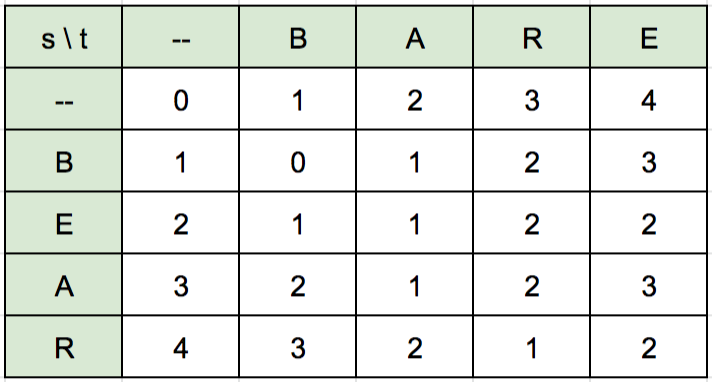
\includegraphics[scale=0.6]{PS10a_Q2.png}
    \end{center}
    \end{figure}
    
    \textbf{Also, draw the alignment corresponding to the arrows} for the given sequences \texttt{s = BEAR} and \texttt{t = BARE} and \textbf{give the set of optimal operations} on the \texttt{s = BEAR} which will transform it to \texttt{t = BARE} (using the cost table with relevant arrows you drew earlier). \\
    An example drawn alignment and set of operations for \texttt{s = STEP} and \texttt{t = APE} look like following. (Show the 'no-op' using a colon (:) to differentiate with a regular sub.)\\\\
    \textbf{Drawn alignment =} $\quad\quad$      \textbf{Ops = }\texttt{['sub', 'sub', 'no-op', 'delete']}
    
    S  T  E  P\\
    $\vert\enspace\enspace\vert\enspace:\thinspace\vert$  \\
    A  P  E  \_\\
    
    \begin{solution}
    Alignment: \\
    
    \pagebreak
    B  E  A  R\\
    $:\enspace\vert\enspace\enspace\vert\enspace\vert$  \\
    B  A  R  E\\
Cost of Alignment: 2
    \end{solution}
    
    \pagebreak
    \item (8 pts) Consider the source sequence \texttt{s = PLAIN}, the target sequence \texttt{t = PLANE}, \texttt{cost(insert) = 2}, \texttt{cost(delete) = 2}, and \texttt{cost(sub) = 2}. Your goal is to align (or transform) the source to the target with minimum cost. Align the source sequence to the target sequence using a bottom-up tabular approach like the one shown on Q2 part b.
    \begin{itemize}
        \item Draw the DP table showing the cost of alignment.
        \item Show the arrows representing the optimal alignment. Note that there are more than one optimal alignment. Show \textbf{two} of the optimal alignments in separate tables using arrows. 
        \\One such example for different sequences and costs - 
        
            \begin{figure}[h!]
            \begin{center}
            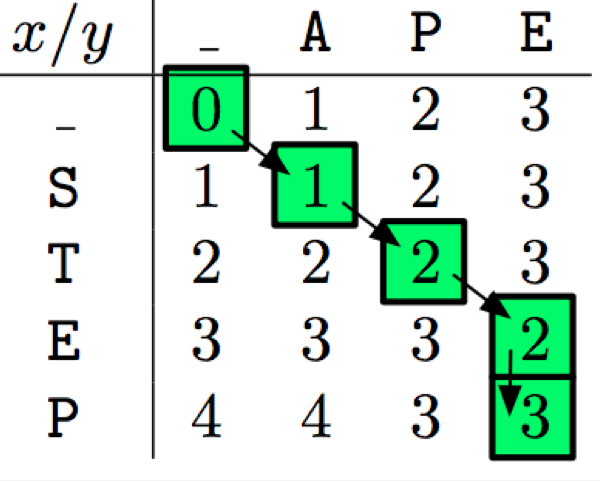
\includegraphics[scale=0.3]{Example.jpeg}
            \end{center}
            \end{figure}
        
        \item Draw the alignments corresponding to the \textbf{two} optimal alignments like you drew in the last part of Q2 part b. 
        \item Provide the cost of the optimal alignment. \\
    \end{itemize}
    
    \begin{solution}
\pagebreak
    \end{solution}
    
    
    
    
\end{enumerate}

\end{enumerate}
\pagebreak



\end{document}

